%!TEX root = thesis.tex

\chapter{Analyse}
\label{chapter-analyse}

\todo[]{Probleme weiter vorne jetzt!!}
Um die relevanten Faktoren und Rahmenbedingungen, die Einfluss auf die Entwicklung und die spätere
Nutzung des Reservierungstools nehmen, identifizieren und einzuordnen zu können wurde eine Analyse
nach dem menschenzentrierten Gestaltungsprozess durchgeführt, um unter anderem Benutzende, Aufgaben
und Kontext des Projektes genauer zu verstehen. Nach einer Ausführung der Datenquellen
(\ref{section:daten}) wurden zunächst zwei Benutzergruppen (Verleihende und Ausleihende) mittels
einer Benutzeranalyse (\ref{section:benutzer}) unter der zu Hilfenahme der durchgeführten Interviews
klassifiziert und eingegrenzt. Anschließend wurden die Aufgaben, die Verleihende und Ausleihende
mithilfe der Anwendung bewältigen möchten, diskutiert (\ref{section:aufgaben}) und der
organisatorische sowie zeitlich-räumliche Kontext des Verleihens und Ausleihens am \ac{imis}
(\ref{section:kontext}) untersucht. Daraufhin wurden die Probleme und Herausforderungen des
aktuellen Vorgehens und unterschiedlichen Ausleihprozesse (\ref{section:iststand}) festgehalten.
Aufbauend auf den Resultaten der vorangestellten Untersuchungen wurden die objektiven Anforderungen
an den SnipeIT Companion formalisiert (\ref{section:anforderung}).

\section{Datenquellen}
\label{section:daten}
\todo[]{Literaturrechereche}
Im Rahmen der Analyse wurden Stakeholder-Interviews durchgeführt und ein vergleichbares Projekt
konnte im Rahmen eines Interviews als weitere Quelle genutzt werden. Die Befragten wurden durch ein
semi-strukturiertes Interview geführt. Im Vorfeld wurde dafür ein Interviewleitfaden entwickelt
(Anhang Verlinken). Es wurde eine Unterteilung in Verleihende und Ausleihende von Assets vorgenommen
(genauere Definition der Benutzergruppen in \ref{section:benutzer}). Bei den Teilnehmenden handelt
es sich um Mitarbeitende, welche am \ac{imis} tätig sind und Studierende der Medieninformatik an der
Universität zu Lübeck. In \ref{table:v} ist der jeweilige (Haupt-)Zuständigkeitsbereich der
Verleihenden aufgeführt. Die Verleihenden der Assets können gleichzeitig die Position eines
Ausleihenden einnehmen. Die Rollen der Ausleihend befragten umfassen sowohl Bachelorstudent als auch
Masterstudenten, diese sind in \ref{table:a} dargestellt. Die IDs der Teilnehmenden werden als
Verweise in den folgenden Abschnitten verwendet\footnote{die mit * gekennzeichneten Personen wurden
gemeinsam interviewt}. Des Weiteren wurde mithilfe des \ac{ati} das technische Interesse und
Verständnis der Teilnehmenden festgestellt, sodass das Reservierungstools entsprechend an die
Benutzergruppen angepasst werden kann \cite{attig_assessing_2017}.


\todo[]{Brauche ich das Alter?}
\begin{table}[h]
        \centering
        \caption{Teilnehmende der Interviews, Verleihende}
        \begin{tabular}{lll}
                \arrayrulecolor{maincolor}\hline
                \sffamily\color{maincolor}ID & \sffamily\color{maincolor}Alter &
                \sffamily\color{maincolor}Zuständigkeitsbereich \\
                \arrayrulecolor{maincolor}\hline
                V1                           & 25 - 35 J.                      & Keine direkte
                Zuständigkeit, Zugänge zu verschiedenen Laboren    \\
                V2                           & 25 - 35 J.                      & Multimedialabor
                \\
                V3                           & 25 - 35 J.                      & VR-Labor
                \\
                V4                           & 40 - 59 J.                      & Administratives
                Personal                                         \\
                V5                           & 25 - 35 J.                      & Innovationslabor
                \\
                \arrayrulecolor{maincolor}\hline
        \end{tabular}
        \label{table:v}
\end{table}

\begin{table}[h]
        \centering
        \caption{Teilnehmende der Interviews, Ausleihende}
        \begin{tabular}{ll}
                \arrayrulecolor{maincolor}\hline
                \sffamily\color{maincolor}ID & \sffamily\color{maincolor}Rolle \\
                \arrayrulecolor{maincolor}\hline
                A1                           & Bachelorstudentin, Hilfswissenschaftlerin
                \\
                A2                           & Bachelorstudent \\
                A3                           & Masterstudent, Hilfswissenschaftler
                \\
                A4*                          & Bachelorstudentin \\
                A5*                          & Bachelorstudentin \\
                A6                           & Masterstudentin \\
                \arrayrulecolor{maincolor}\hline
        \end{tabular}
        \label{table:a}
\end{table}

\section{Benutzeranalyse}
\label{section:benutzer}
Um eine zielgruppengerecht Gestaltung des SnipeIT Companion voraussetzten zu können, werden in
diesem Abschnitt die Benutzergruppen des Reservierungstools eruiert und näher untersucht.
Resultierend aus den Stakeholder-Interviews wurden zwei Benutzergruppen, zu denen Verleihende sowie
Ausleihende eines Assets gehören, für das System erarbeitet.

Aus den Interviews (\ref{section:daten}) konnte zudem entnommen werden, dass beide Benutzergruppen
täglich ein Smartphone, Tablet, Laptop oder Desktop PC nutzen und somit ein grundlegendes
technisches Verständnis vorausgesetzt werden kann. Diese Behauptung konnte mit den Ergebnissen der
\ac{ati}-Skala bestärkt werden (\ref{table:ati}).

\begin{table}[h]
        \centering
        \caption{Ergebnisse der \ac{ati}-Skala}
        \begin{tabular}{ll}
                \arrayrulecolor{maincolor}\hline
                \sffamily\color{maincolor}Mittelwert & \sffamily\color{maincolor}Blaa
                \\
                \arrayrulecolor{maincolor}\hline
                Zahl                                 & Dinge \\
                \arrayrulecolor{maincolor}\hline
        \end{tabular}
        \label{table:ati}
\end{table}


\subsection*{Verleihende}
Mitarbeitende, sowie administratives Personal des \ac{imis}, welche verantwortlich für das Verleihen
von Assets sind, werden im folgenden als Verleihende bezeichnet (\ref{table:v}). Verleihende sind in
der Lage, einzelne Assets herauszugeben, allerdings haben nicht alle Verleihende auf alle Assets den
gleichen Zugriff, dies ist von Forschungsgruppe zu Forschungsgruppe unterschiedliche und umfasst
zudem unterschiedliche Vorgänge (genauere Unterschiede zu den Vorgängen in \ref{section:iststand}).
Folglich können Verleihenden der Assets gleichzeitig die Position der Ausleihenden einnehmen.

\subsection*{Ausleihende}
% Was schreibe ich da noch groß zu?
Bei den Ausleihenden handelt es sich insbesondere um Studierende, welche keinen direkten Zugang zu
den Assets haben, diese aber Ausleihen können (\ref{table:a}). Mitarbeitende, welche von anderen
Forschungsgruppen ein Asstet ausleihen wollen haben häufig einen anderen Ausleihprozess als
Studierende, da der Vertrauens- und Bekanntheitsgrad ein anderer ist (V1,V2,V3).

\todo[inline]{Im Rahmen der Arbeit wird der Fokus auf die Ausleihenden gelegt. Aus den und den
        Gründen. Dadurch fallen aber auch bestimmte Punkte für Verleihende an.}

\todo[inline]{Die Zielgruppe besteht hauptsächlich aus Mitarbeitenden des \ac{imis} sowie
        Studierenden.}

\section{Problemanalyse}
\label{section:iststand}
        
Um die Probleme des Ausleihens am \ac{imis} nachvollziehen zu können, wurde im folgenden eine
Problemanalyse auf Basis der Interview aussagen getroffen. 
Der Übersichtlichkeit werden im Folgenden Probleme, welche Verleihende und Ausleihende betreffen zu
erst Thematisiert. Daraufhin werden Probleme der einzelnen Benutzergruppen näher erläutert.

\subsection*{Probleme: Allgemein}
Aus den Interviews konnte gefolgert werden, dass keine öffentlichen Listen für Studieren über die
Assets einsehbar sind. Gleichzeitig wurde erarbeitet, dass auch keine vollständigen intenren Listen
oder Übersichten am \ac{imis} vorhanden sind (V,A). Dies führt dazu, dass beiden Nutzergruppen nicht
bekannt ist, was ausleihbar ist (alle). Es kommt zu einem häufigerem weiterverweisen, an andere
Personen, weil kein direkter Ansprechpartner ersichtlich ist (V1,V3, V4, A1, A2, A3). Da es aus Seiten
der \ac{hiwi} und der \ac{wimi} zu Vorkommnissen kam, bei denen Assets kurzzeitig, ohne Vermerk
genommen wurden, ... (A1, V1, V2). Das Ausleihen unter den \ac{hiwi} und \ac{wimi} läuft häufig auf
Vertrauenbasis; Kein Verzeichnis von Gebrauchsspuren (A1, V1,)

Selbstaneignung (V1, V4, V5, A3) Studierende kommen ohne wissen 

Je nach dem, wieviel Wissen Ausleihende haben Usecase..(V2, A6)

\subsection*{Probleme: Verleihende}
Eine zentrale Schwachstelle des aktuellen Prozesses ist es, das es keinen einheitlichen Prozesses
gibt. Das Ausleihen von Assets wird von Forschungsgruppe zu Forschungsgruppe unterschiedliche
gehandhabt, bzw. innerhalb der Forschungsgruppe gibt es je nach Verleihenden auch wieder
unterschiede im Prozess (V1, V2,V3). Während Verleihenden wichtig ist, dass Ausleihende über die
Assets Bescheid wissnen und der Usecase detailliert besprochen und erläutert wird, ist die
Vermittlung dieses Wissens nicht von Bedeutung. \\
Überleitung finden\\
Zettelwirtschaft (V4, V5) Unterschrift auf irgendeinem Zettel (V1, V2, V3, V4) Häufig nicht
dokumentiert (V1, V2). Was passiert, wenn es kaputt geht? Absicherung, Transparenz, bekannte Macken
klar? -> nein (alle V)

Auf Seiten ist das nichtvorhanden sein einer Übersicht der Verfügbaren Assets insofern gravierend,
als dass es durch die Unwissenheit zu Doppelbeschaffung kommen kann (V1, V2, V3). Außerdem kann es
dazu kommen, das Material beschaffts wird, welches mit dem Vorhanden nicht kompatible ist (V2,V3).

2 Jahre nicht gewusste, wo ein Teil liegt, dabei war es gefühlt im Raum neben an ... hätte die
Arbeit bei einem verangenen Projekt sehr erleichert (V2).

Es ist kein sponatens planen (V1, V2, V3, ...) und für Studien schwer

Fragen nach "Kamera" -> Nachfragen, was sie brauchen und helfen -> Gespräch komplex (V2) 

Keine Wartung oder Person, die sich so richtig verantortlich fühlt, bzw. die Person die es gekauft
hat ist zuständig,... Akku leer, ... nicht vernünftig zurückgelegt ()

\subsection*{Probleme: Ausleihende}
% Verantwortlichkeiten unklar (für Studierende) (A1, A2, A5)
Über Flurfunk oder Videoworkshop aber nicht über alles bescheid (alle As) Aber auch: entspannt aber
nicht klar, was ausleihende ist (A4, A5). Unzuverlässlig (spontanes Planen schwierig), weil... (A1,
A6). Keine Garantie, dass es etwas zu bestimmten Punkten da ist (A1, A3) kein Schnelles Herankommen,
weil an Person angewiesen sind (A3). Spontane nachfragen nach Assets sind eher weniger häufig
aufseiten der Studierenden zu sehen, hier wird vorher eher eine Mail an einen \ac{wimi}, in den
Meisten Fällen an die Verantwortlichen Übungsleiter oder die Studiengangskoordination, schreiben,
weil Riskio zu hoch, das Asset schon weg ist (A3). Stark kritisiert wird hier, dass das nachfragen
als sehr nervig wahrgenommen wird, weil jemand aus der Arbeit gerissen wird (A6). Dazu kommt, dass
Ausleihene häufig nicht genau wissen um was für ein Gerät es genau handelt, so kann es zu
kompatiblitätsfehlern kommen Auskunft fehlt (Selbstaneignung) (A3), Projekt konnte am Ende aber
nicht mit dem Asset umgesetzt werden (A3). 


\section{Aufgabenanalyse}
\label{section:aufgaben}
Durch die Aufgaben, welche Verleihende und Ausleihende im Ausleihprozess durchlaufen, konnte
Resultierend auf Basis der Interviews (\ref{section:daten}) Aufgaben erarbeitet werden, welche von
dem Reservierungstools übernommen oder unterstützt werden können. Die Aufgaben wurden anhand des
Ausleihprozesses in drei Bereiche eingeordnet. Im ersten Bereich handelt es sich um die
Vorbereitung, welche zum Ausleihen eines Assets getroffen werden müssen, darauffolgend werden die
Aufgaben der Ausgabe definiert. Der dritte Bereich umfasst die Rückgabe der Assets. Ergänzend zu den
zuvor gehenden Aufgaben und Interviews zu den drei Bereichen wurden Aufgaben für die Wartung der
Assets dargestellt.

% 1. Überschrift ausgeführt 2. wer und besonderheiten (Zielgruppe) 3. Rahmenbediungen 4. Details

% Aufgabe im Bereich der Vorbereitung
\subsection*{Aufgaben im Bereich der Vorbereitung}
Zunächst wird auf die Vorbereitungen eingegangen, welche getroffen werden müssen, bevor ein Asset
ausgeliehen bzw. abgeholt werden kann.
\subsubsection*{Ag-Vt-1 | Übersicht über ausleihbare Assets}
Wie bereits in der Problemanalyse () gab es zum Zeitpunkt der Interviews keine Übersicht, über
Assets. Dies zeigt die Dringlichkeit des SnipeIT Companion für eine besser Vorbereitung. So
können Ausleihende mit mehr Wissen eine Anfragen zum Ausleihen stellen. 
\subsubsection*{Ag-Vt-2 | Checkliste/Dialog für Vorschläge}
Um den Ausleihprozess für Verleihende zu erleichtern kann der Vorangestellt Usecase mittelts eines
Dialogs ermöglicht werde. So können aufbauend darauf, direkt Vorschläge an Ausleihende gegeben werden.
\subsubsection*{Ag-Vt-3 | Verfügbarkeit von Assets einsehen}
Um ein Assets ausleihen zu können ist es sowohl für Verleihende als auch Ausleihende von bedeutung, 
ob Assets Verfügbar sind
\subsubsection*{Ag-Vt-4 | Reservierungen von Assets}
Durch die Verfügbarkeit können wir Reservieren
\subsubsection*{Ag-Vt-5 | Kalenderübersicht}
Anknüpfend an Ag-Vt-3 und Ag-Vt-4 ist eine ... sinnvoll.
\subsubsection*{Ag-Vt-6 | Sichtbarkeit von Ansprechpartner:innen}
Nicht ersichtlich aktuell, Fragen im Voraus 

% Aufgabe der Ausgabe 
\subsection*{Aufgaben im Bereich der Ausgabe}
Im nächsten Abschnitt werden alle Zentralen Aufgaben aufgeführt, welche für die Übergabe von
Verleihnden zu Ausleihnden umfasst.
\subsubsection*{Ag-Au-1 | Zugang zu Assets}
Damit Ausleihen die gewünschten Assets aus den Laboren entnehmen können, müssen Verleihende
die Entsprechenden Räumlichkeiten aufschließen. Hierbei ist zu berücksichtigen, dass die
Forschungsgruppe untereinander auch nicht immer Zugriff haben (Verweis:Ansprechpartner Ag-Vt-6).
\subsubsection*{Ag-Au-2 | Kommunikationsmöglichkeit bieten}
?
\subsubsection*{Ag-Au-3 | Vermittlung/Nutzung von Assets erläutern}
Ausleihene wissen vorher häufig nicht genau um was für ein Gerät es genau handelt, so kann es zu
kompatiblitätsfehlern kommen und das Asset ist für den Usprübglichen Gebauch nicht nutzbar.
Daher ist eine Übersicht mit Informationen wie: Seriennummer,... sowie der dazugehörigen Anleitung sinnvoll.
\subsubsection*{Ag-Au-4 | Ausgeliehene Assets dokumentieren}
?
\subsubsection*{Ag-Au-5 | Rechtliche Rahmenbedingungen}
Durch die uneinheitlichen Vorgänge, sind die Verantwortlichkeiten häufig nicht immer klar. (Forschungsgruppe..)
Daher... 
Da die Assets nicht versichert sind, läuft das Ausleihen auf Vertrauenbasis. Sollten Krasser oder
weitere Schäden entstehen vereinbaren Nutzenden somit, diese direkt zu melden.

% Aufgaben der Rückgabe
\subsection*{Aufgaben im Bereich der Rückgabe}
Die Nachfolgenden Aufgaben umfassen die Rückgabe der Ausgeliehenen Assets.

\subsubsection*{Ag-Rg-1 | Erinnerungen erhalten}
Kann ja vorkommen, dass mal was vergessen wird...
\subsubsection*{Ag-Rg-2 | Assets korrekt zurückgebracht}
Akkus voll, SD karte leeren, Ursprüngliche Einstellungen,...

% Aufgaben der Wartung
\subsection*{Aufgaben im Bereich der Wartung}
Im Folgenden werden Aufgaben, welche für Verleihende auf Administariver Ebene von Bedeutung sind
näher erläutert. 

\subsubsection*{Ag-Wt-1 | Pflege von Assets}
Updates nach langer Nicht Nutzung, Akuus entladen,...

\subsubsection*{Ag-Wt-2 | Pflege der Datenbank/Übersicht/Liste}
Bei Neuanschaffung, keinen Überblick über die Erneuerungen, ...



\section{Kontextanalyse}
\label{section:kontext}

Um zu ermitteln, in welcher Nutzungsumgebung die Anwendung verwendet werden soll, wurde eine
Kontextanalyse durchgeführt.

\subsection*{Organisatorischer Kontext}
Innerhalb des Universitäts-Kontextes gibt es aus formaler Sicht eine überwiegend flache Hierarchie
zwischen Studierenden und Mitarbeitenden, wobei zwischen Hilfswissenschaftlern und
Hilfswissenschaftlerinnen, wissenschaftlichen Mitarbeitenden sowie Professoren und Professorinnen
unterschieden werden kann. Diese Gruppen haben teilweise unterschiedlichen Zugriff auf bestimmte
Systeme wie einen Kalender, in dem Mitarbeitende die belegten Zeiten von Kollegen einsehen können.

Aus informeller Sicht ist die Verbindung zwischen Mitarbeitenden und den Personen, die das Büro
aufsuchen, meist kollegial (z.B. bei anderen Mitarbeitenden) oder situativ (z.B. bei Studierenden).

\subsection*{Zeitlich-Räumlicher Kontext}
\label{section:zeit}
Der Kontext sollte sowohl aus Sicht der Verleihenden als auch aus Sicht der Ausleihenden analysiert
werden. Die Anwendung soll einen einheitlichen Ausleihprozess schaffen. Mitarbeitende halten sich
entweder in ihren Büros oder an einem anderen Ort auf, daher werden bei der Analyse des
zeitlich-räumlichen Kontextes beide Fälle betrachtet.

Befindet sich Mitarbeitende im Büro, arbeiten sie an einem Desktop-Arbeitsplatz. Der Computer ist
dabei die meiste Zeit eingeschaltet, häufig arbeiten Mitarbeitende am Computer, beispielsweise in
Form einer Web-App an, da der Aufwand zur Bedienung dieser Web-App gering ist (...). Wenn
Mitarbeitende aus diversen Gründen ihr Büro verlassen, stehen sie auf und schließen beim Hinausgehen
die Bürotür.

Die Bedienung der Anwendung sollte daher sehr niedrigschwellig sein, da Mitarbeitende häufig nicht
viel Zeit für die Bedienung haben oder investieren möchten (...).

Da der Ort variiert, liegt hier ein mobiler Nutzungskontext vor, welches beispielsweise durch die
Nutzung einer Web-App auf dem Smartphone ermöglicht werden kann (V1, V2, V , A).

%Wie eingangs er-wähnt, definieren die Anforderungen, was das System zu leisten hat, während die
%Funktionalitä-ten definieren, wie das System diese gewährleistet.

\section{Formalisierte Anforderungen}
\label{section:anforderung}

Im Folgenden werden systematisch formalisierte Anforderungen präsentiert, welche die Ergebnisse der
Analysen abschließend zusammenfassen. Es werden zunächst die Visionen und Ziele
(\ref{section:visionziel}) definiert, des Weiteren werden die Rahmenbedingungen
(\ref{section:rahmen}) und der Kontext des Systems (\ref{section:kontextueberblick}) dargestellt.
Darauf aufbauend wird eine funktionale Anforderung erstellt (\ref{section:funktionale}). Abschließen
werden die Qualitätsanforderungen formuliert (\ref{section:qualität}).


\subsection*{Vision und Ziele}
\label{section:visionziel}
Zunächst werden die Visionen und Ziele des Systems konkretisiert, an denen sich die Anforderungen
auf Zielgerichtetheit überprüfen lassen \cite{balzert2009}. Diese setzen sich aus der Analyse der
Benutzenden sowie Aufgaben und des Kontextes zusammen. Im ersten Schritt werden die Visionen für die
Zukunft realitätsnah festgelegt.



\begin{center}
        \renewcommand{\arraystretch}{1.5}
        \begin{tabular}{p{0.1\textwidth}p{0.8\textwidth}}
                \hline
                \textbf{/V10/} & Verleihende \\
                \textbf{/V20/} & Ausleihende haben wissen, über auszuleihende Assets.
                \\
                \hline
        \end{tabular}
\end{center}

Basierend auf diese Visionen lassen sich die Ziele formulieren, welche die Visionen
operationalisieren. Diese folgen dabei den standardisierten Regeln zur Formulierung von Zielen
\cite{pohl_requirements_2008}.


\begin{center}
        \renewcommand{\arraystretch}{1.5}
        \begin{tabular}{p{0.1\textwidth}p{0.8\textwidth}}
                \hline
                \textbf{/Z10/} & Ausleihende eines Assets erhalten zielgerichtete und aktuelle
                Informationen zum Verbleib. \\
                \textbf{/Z20/} & Ausleihende sind jederzeit in der Lage, . \\
                \textbf{/Z40/} & XX sind überall in der Lage, ihre Informationen zu ändern.
                \\
                \textbf{/Z50/} & . \\
                \hline
        \end{tabular}
\end{center}

\subsection*{Rahmenbedingungen}
\label{section:rahmen}
Die Randbedingungen legen organisatorische und technische Restriktionen für das System oder den
Entwicklungsprozess fest \cite{balzert2009}. Die Bedingungen wurden aus der Benutzer- und
Kontextanalyse abgeleitet.

\begin{center}
        \renewcommand{\arraystretch}{1.5}
        \begin{tabular}{p{0.1\textwidth}p{0.8\textwidth}}
                \hline
                \textbf{/R10/} & Das System ist eine Web-Anwendung. \\
                \textbf{/R20/} & Die Zielgruppe sind Mitarbeitende des IMIS und Studierende.
                \\
                \textbf{/R30/} & Die Zielgruppe teilt sich in zwei Nutzergruppen: die Verleihenden
                und Ausleihende von Assets. Die Definitionen der Nutzergruppen sind in Kapitel
                (\secref{section:benutzer}) zu finden. \\
                \textbf{/R40/} & Das System wird von Verleihenden sowohl im mobilen als auch im
                ...Kontext genutzt. \\
                \textbf{/R50/} & Die eingesetzte Software auf der Zielmaschine ist clientseitig ein
                Webbrowser. Die marktführenden Webbrowser müssen unterstützt werden: Chrome,
                Firefox, Safari \cite{noauthor_browser_nodate}. \\
                \hline
        \end{tabular}
\end{center}

\subsection*{Kontext und Überblick}
\label{section:kontextueberblick}
Ein System ist in einer technischen Umgebung eingebettet \cite{balzert2009}. Es wurde im folgenden
Bezug auf das aktuelle Vorgehen mithilfe der Problemanalyse geschlossen.

\begin{center}
        \renewcommand{\arraystretch}{1.5}
        \begin{tabular}{p{0.1\textwidth}p{0.8\textwidth}}
                \hline
                \textbf{/K10/} & Das aktuelle Vorgehen umfasst keine Liste für Verleihende und
                Ausleihende. \\
                \textbf{/K20/} & Es kommmt zu Doppelbeschaffungen. \\
                \textbf{/K30/} & Es existieren von Forschungsgruppe zu Forschungsgruppe
                unterschiedliche Ausleihprozesse. \\
                \hline
        \end{tabular}
\end{center}

\subsection*{Funktionale Anforderungen}
\label{section:funktionale}
Im Folgenden werden die Kernfunktionalitäten des Systems aufgeführt \cite{balzert2009}. Diese
ergeben sich aus der Aufgabenanalyse (\ref{section:aufgaben}). Um die Anforderungen mit einer
eindeutigen Semantik zu formulieren, wurde eine Anforderungsschablone (\ref{fig:schablone})
verwendet, um natürlichsprachliche Anforderungen zu definieren \cite{balzert2009}.

\begin{figure}[h]
        \centering
        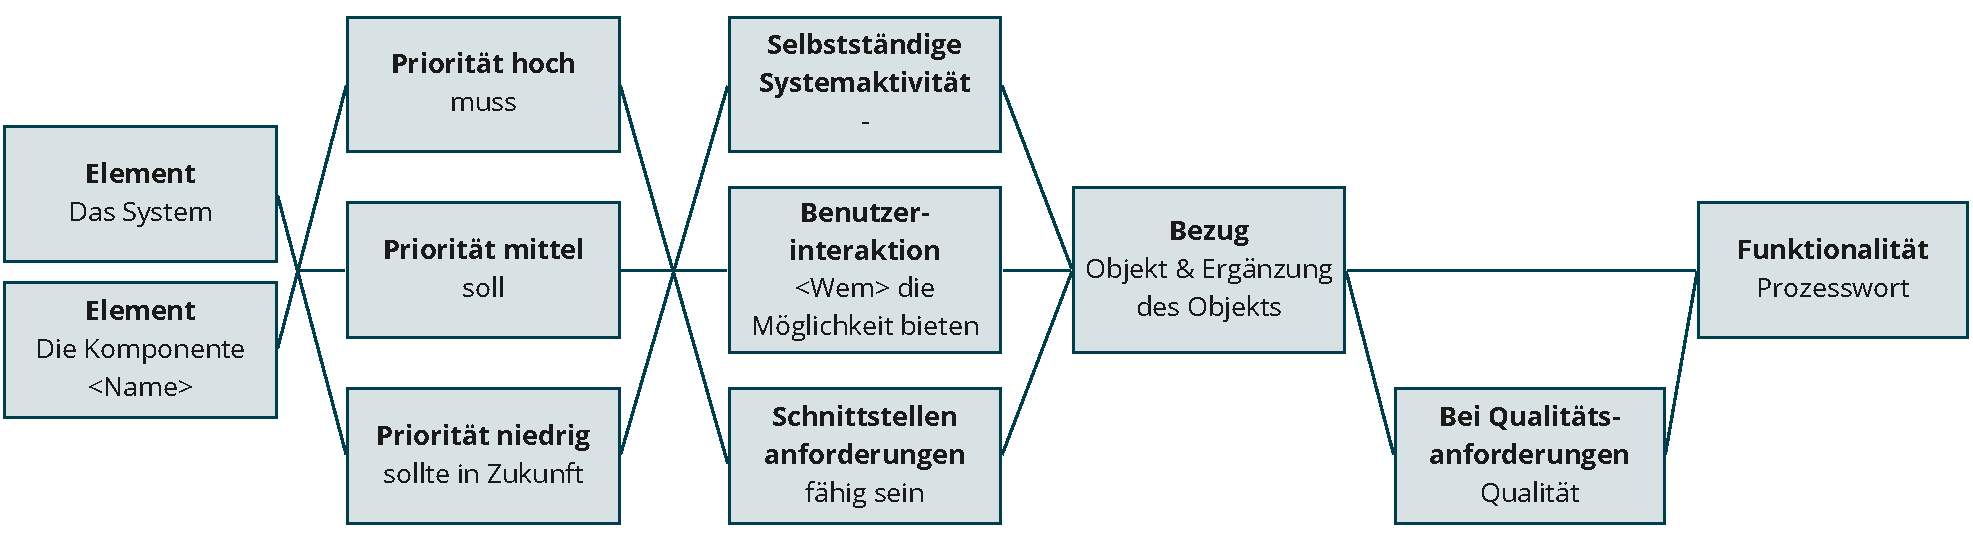
\includegraphics[scale=0.45]{Bilder/anforderungsschablone.pdf}
        \label{fig:schablone}
        \caption[Anforderungsschablone]{Anforderungsschablone \cite{balzert2009}}
\end{figure}


\begin{center}
        \renewcommand{\arraystretch}{1.5}
        \begin{tabular}{p{0.1\textwidth}p{0.8\textwidth}}
                \hline
                \textbf{/F10/}  & Das System \textit{muss} Verleihenden und Ausleihenden die
                Möglichkeit bieten, eine Übersicht der Assets jederzeit einsehen zu können (A).
                \\
                \textbf{/F20/}  & Das System \textit{muss} XX die Möglichkeit bieten,  .
                \\
                \textbf{/F30/}  & Das System \textit{muss} XX die Möglichkeit bieten,  (A).
                \\
                \textbf{/F40/}  & Das System \textit{muss} XX relevante Informationen anzeigen, (A).
                \\
                \textbf{/F50/}  & Das System \textit{muss} XX die Möglichkeit geben,.
                \\
                \textbf{/F60/}  & Das System \textit{soll} die Möglichkeit bieten, individuelle und
                personalisierte Inhalte zu visualisieren -> Checkliste (A).
                \\
                \textbf{/F70/}  & Das System \textit{soll} daran erinnern, die Ausgeliehenen Assets
                zurückzubringen oder zu verlängern oder abzuholen (A).
                \\
                \textbf{/F80/}  & Das System \textit{soll} XX die Möglichkeit bieten, .
                \\
                \textbf{/F90/}  & Das System \textit{sollte in Zukunft} . \\
                \textbf{/F100/} & Das System \textit{sollte in Zukunft} XX die Möglichkeit bieten,
                Informationen zu hinterlassen (A). \\
                \textbf{/F110/} & Das System \textit{sollte in Zukunft} . \\
                \hline
        \end{tabular}
\end{center}


\subsection*{Qualitätsanforderungen}
\label{section:qualität}
Im letzten Schritt werden die nicht-funktionalen Anforderungen festgelegt, welche die qualitativen
oder quantitativen Eigenschaften eines Systems darstellen \cite{balzert2009}. Auch hier wird, falls
möglich, die Anforderungsschablone aus \ref{fig:schablone} verwendet.

\begin{center}
        \renewcommand{\arraystretch}{1.5}
        \begin{tabular}{p{0.1\textwidth}p{0.8\textwidth}}
                \hline
                \textbf{/Q10/} & Das System \textit{muss} den Grundsätzen der DIN EN ISO
                9241-110:2019-09 (Ergonomie der Mensch-System-Interaktion - Teil 110:
                Interaktionsprinzipien) folgen (\textit{DIN EN ISO 9241-110}, 2019).
                \\
                \textbf{/Q20/} & Das System \textit{muss} die definierten Nutzungsklassen aus
                \ref{section:benutzer} unterscheiden und die dazugehörigen Zugriffsrechte
                sicherstellen. \\
                \textbf{/Q30/} & Das System \textit{soll} modular strukturiert sein, damit Inhalte
                und Funktionalitäten effizient eingebunden werden können und das System einfach
                erweiterbar ist. \\
                \textbf{/Q40/} & Das System \textit{soll} beim Zugriff über das Internet eine
                gesicherte Übertragung (bspw. \ac{HTTPS}) ermöglichen.
                \\
                \textbf{/Q50/} & Das System \textit{soll} alle Benutzerinteraktionen in unter fünf
                Sekunden ausführen. \\
                \hline
        \end{tabular}
\end{center}
